یک سرویس \lr{HTTP} به زبان \lr{Go 1.23} با دو API \lr{GET /health} و \lr{POST /v1/analyze} (آمار واژگان یک متن) نوشته شد؛ ۱۵ تست واحد با پوشش ۷۰ درصدی کل و ۱۰۰ درصدی بسته‌ی منطق دامنه. تنها وابستگی بیرونی \lr{github.com/google/uuid} است تا مرحله‌ی \lr{install} کار واقعی داشته باشد. سرویس \lr{graceful shutdown} دارد و شماره‌ی نسخه‌اش در زمان بیلد با \lr{-ldflags} روی باینری حک می‌شود؛ همین باعث می‌شود در مرحله‌ی \lr{deploy} بتوان تأیید کرد که دقیقا همان \lr{artifact} این پایپلاین اجرا شده است.


چون \lr{GitLab Runner} نداریم، اسکریپت \lr{runner.bash} نقش آن را بازی می‌کند. هر جاب دقیقا مثل \lr{docker executor} در یک کانتینر یک‌بارمصرف اجرا می‌شود:

\begin{lstlisting}[language=bash]
in_docker() {
    local image="$1"; shift
    docker run --rm \
        -v "$WORKSPACE:/src" \
        -v "$ARTIFACTS_DIR:/artifacts" \
        -v "$MOD_CACHE_VOL:/go/pkg/mod" \
        -v "$BUILD_CACHE_VOL:/root/.cache/go-build" \
        -w /src -e CGO_ENABLED=0 -e GOFLAGS=-buildvcs=false \
        "$image" sh -eu -c "$*"
}
\end{lstlisting}

دو جابی که باید خود \lr{daemon} را صدا بزنند (\lr{build} و \lr{deploy}) نسخه‌ی دومی از همین تابع را استفاده می‌کنند که \lr{/var/run/docker.sock} را هم \lr{mount} می‌کند — همان الگویی که رانرهای واقعی برای ساخت ایمیج به‌کار می‌برند.

\begin{center}
\begin{tabular}{|l|l|l|}
\hline
{جاب} & {ایمیج} & {کار و شرط عبور} \\
\hline
\lr{install} & \lr{golang:1.23-alpine} & \lr{go mod download} و \lr{go mod verify} \\
\hline
\lr{lint} & \lr{golang:1.23-alpine} + & \lr{gofmt -l}، \lr{go vet}، سپس \lr{golangci-lint} \\
 & \lr{golangci-lint:v1.62.2} & (\lr{errcheck}، \lr{staticcheck}، \lr{revive} و ...) \\
\hline
\lr{build} & \lr{golang} + \lr{docker:27-cli} & باینری ایستا به‌عنوان \lr{artifact}، سپس ساخت ایمیج \\
\hline
\lr{test} & \lr{golang:1.23-alpine} & \lr{go test -race} با گزارش پوشش \\
\hline
\lr{deploy} & \lr{docker:27-cli} + \lr{alpine} & استقرار ماک و \lr{smoke test} \\
\hline
\end{tabular}
\end{center}

\lr{deploy} به این صورت ماک است که یک شبکه‌ی موقت می‌سازد، ایمیج همین پایپلاین را روی آن بالا می‌آورد، از یک کانتینر {دیگر} روی همان شبکه \lr{/health} و \lr{/v1/analyze} را صدا می‌زند و در پایان چه موفق و چه ناموفق با یک \lr{trap} محیط را آزاد می‌کند. یعنی چیزی واقعا اجرا و آزموده می‌شود، ولی هیچ محیط پایداری درگیر نمی‌شود.

 امکاناتی که از \lr{GitLab CI} تقلید شده‌اند:

\begin{itemize}
	\item {کش}: دو \lr{volume} به نام‌های \lr{q7-go-mod-cache} و \lr{q7-go-build-cache} بین اجراها باقی می‌مانند (معادل \lr{cache:}).
	\item {\lr{artifact}}: باینری، \lr{coverage.out} و \lr{coverage.html} در \lr{.ci/artifacts/} و لاگ جداگانه‌ی هر جاب در \lr{.ci/logs/}.
	\item {\lr{dotenv} بین جاب‌ها}: جاب \lr{build} تگ ایمیجی که ساخته را در \lr{build.env} می‌نویسد و \lr{deploy} همان را می‌خواند؛ معادل \lr{artifacts:reports:dotenv}. بدون این، \lr{deploy} نمی‌داند کدام ایمیج را مستقر کند.
	\item {\lr{fail-fast}}: اولین جاب شکست‌خورده باعث می‌شود بقیه \lr{skipped} علامت بخورند و کد خروج اسکریپت غیرصفر شود.
	\item {\lr{allow\_failure}}: فهرستی از جاب‌ها که شکستشان پایپلاین را متوقف نمی‌کند (فعلا خالی).
	\item {اجرای گزینشی}: \lr{./runner.bash lint test} فقط همان جاب‌ها را اجرا می‌کند.
\end{itemize}

 نتیجه‌ی اجرا در حالت موفق:

\begin{figure}[H]
\centering
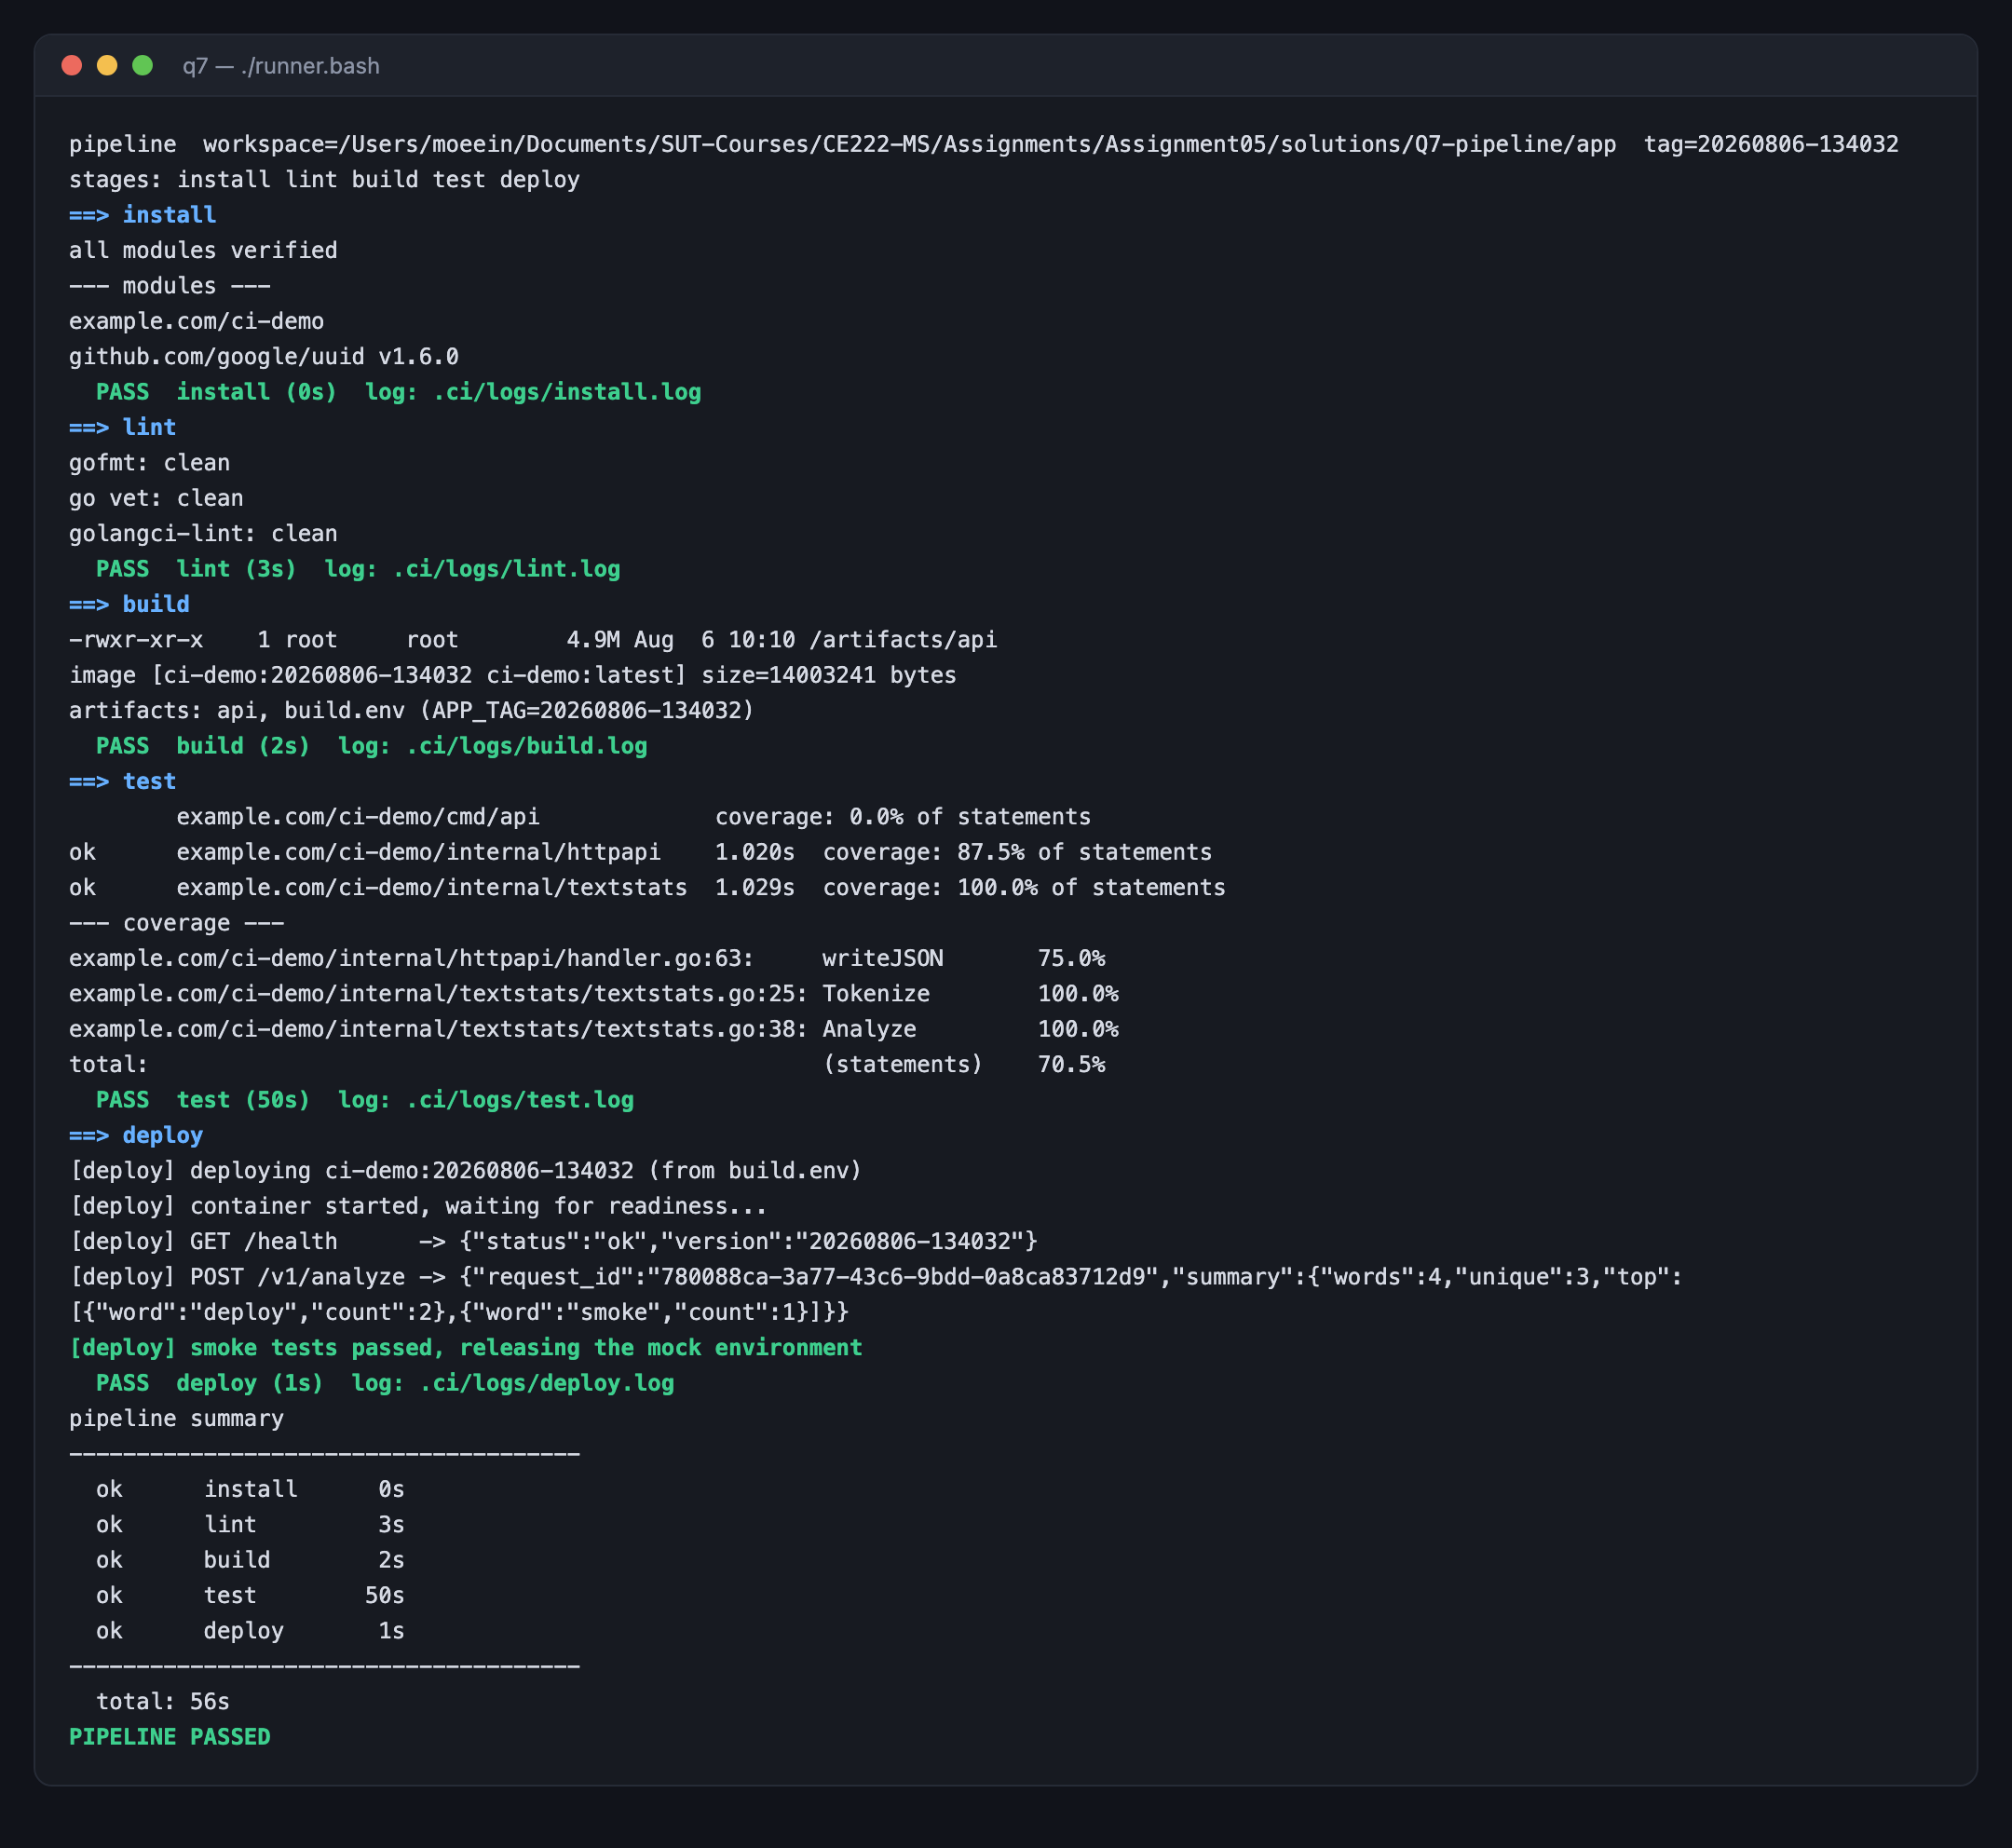
\includegraphics[width=0.95\textwidth]{figs/q7-pass.png}
\caption{اجرای کامل \lr{./runner.bash}؛ همه‌ی پنج جاب سبز و کد خروج صفر.}
\end{figure}

نتیجه‌ی اجرا در حالت شکست:

برای اینکه نشان دهیم هر دروازه واقعا مسدود می‌کند، اسکریپت \lr{demo-failure.bash} پروژه را در یک پوشه‌ی موقت کپی می‌کند، یک نقص {واقعی} تزریق می‌کند و پایپلاین را روی همان کپی اجرا می‌کند (سورس اصلی دست‌نخورده می‌ماند):

\begin{center}
\begin{tabular}{|l|l|}
\hline
{مرحله} & {نقص تزریق‌شده} \\
\hline
\lr{lint} & فایلی با قالب‌بندی نادرست و یک خطای بررسی‌نشده \\
\hline
\lr{build} & \lr{COPY} از فایلی که وجود ندارد در \lr{Dockerfile} \\
\hline
\lr{test} & تغییر یک انتظار در تست واحد \\
\hline
\lr{deploy} & \lr{LISTEN\_ADDR} نامعتبر، پس سرویس هرگز سالم نمی‌شود \\
\hline
\end{tabular}
\end{center}

\begin{figure}[H]
\centering
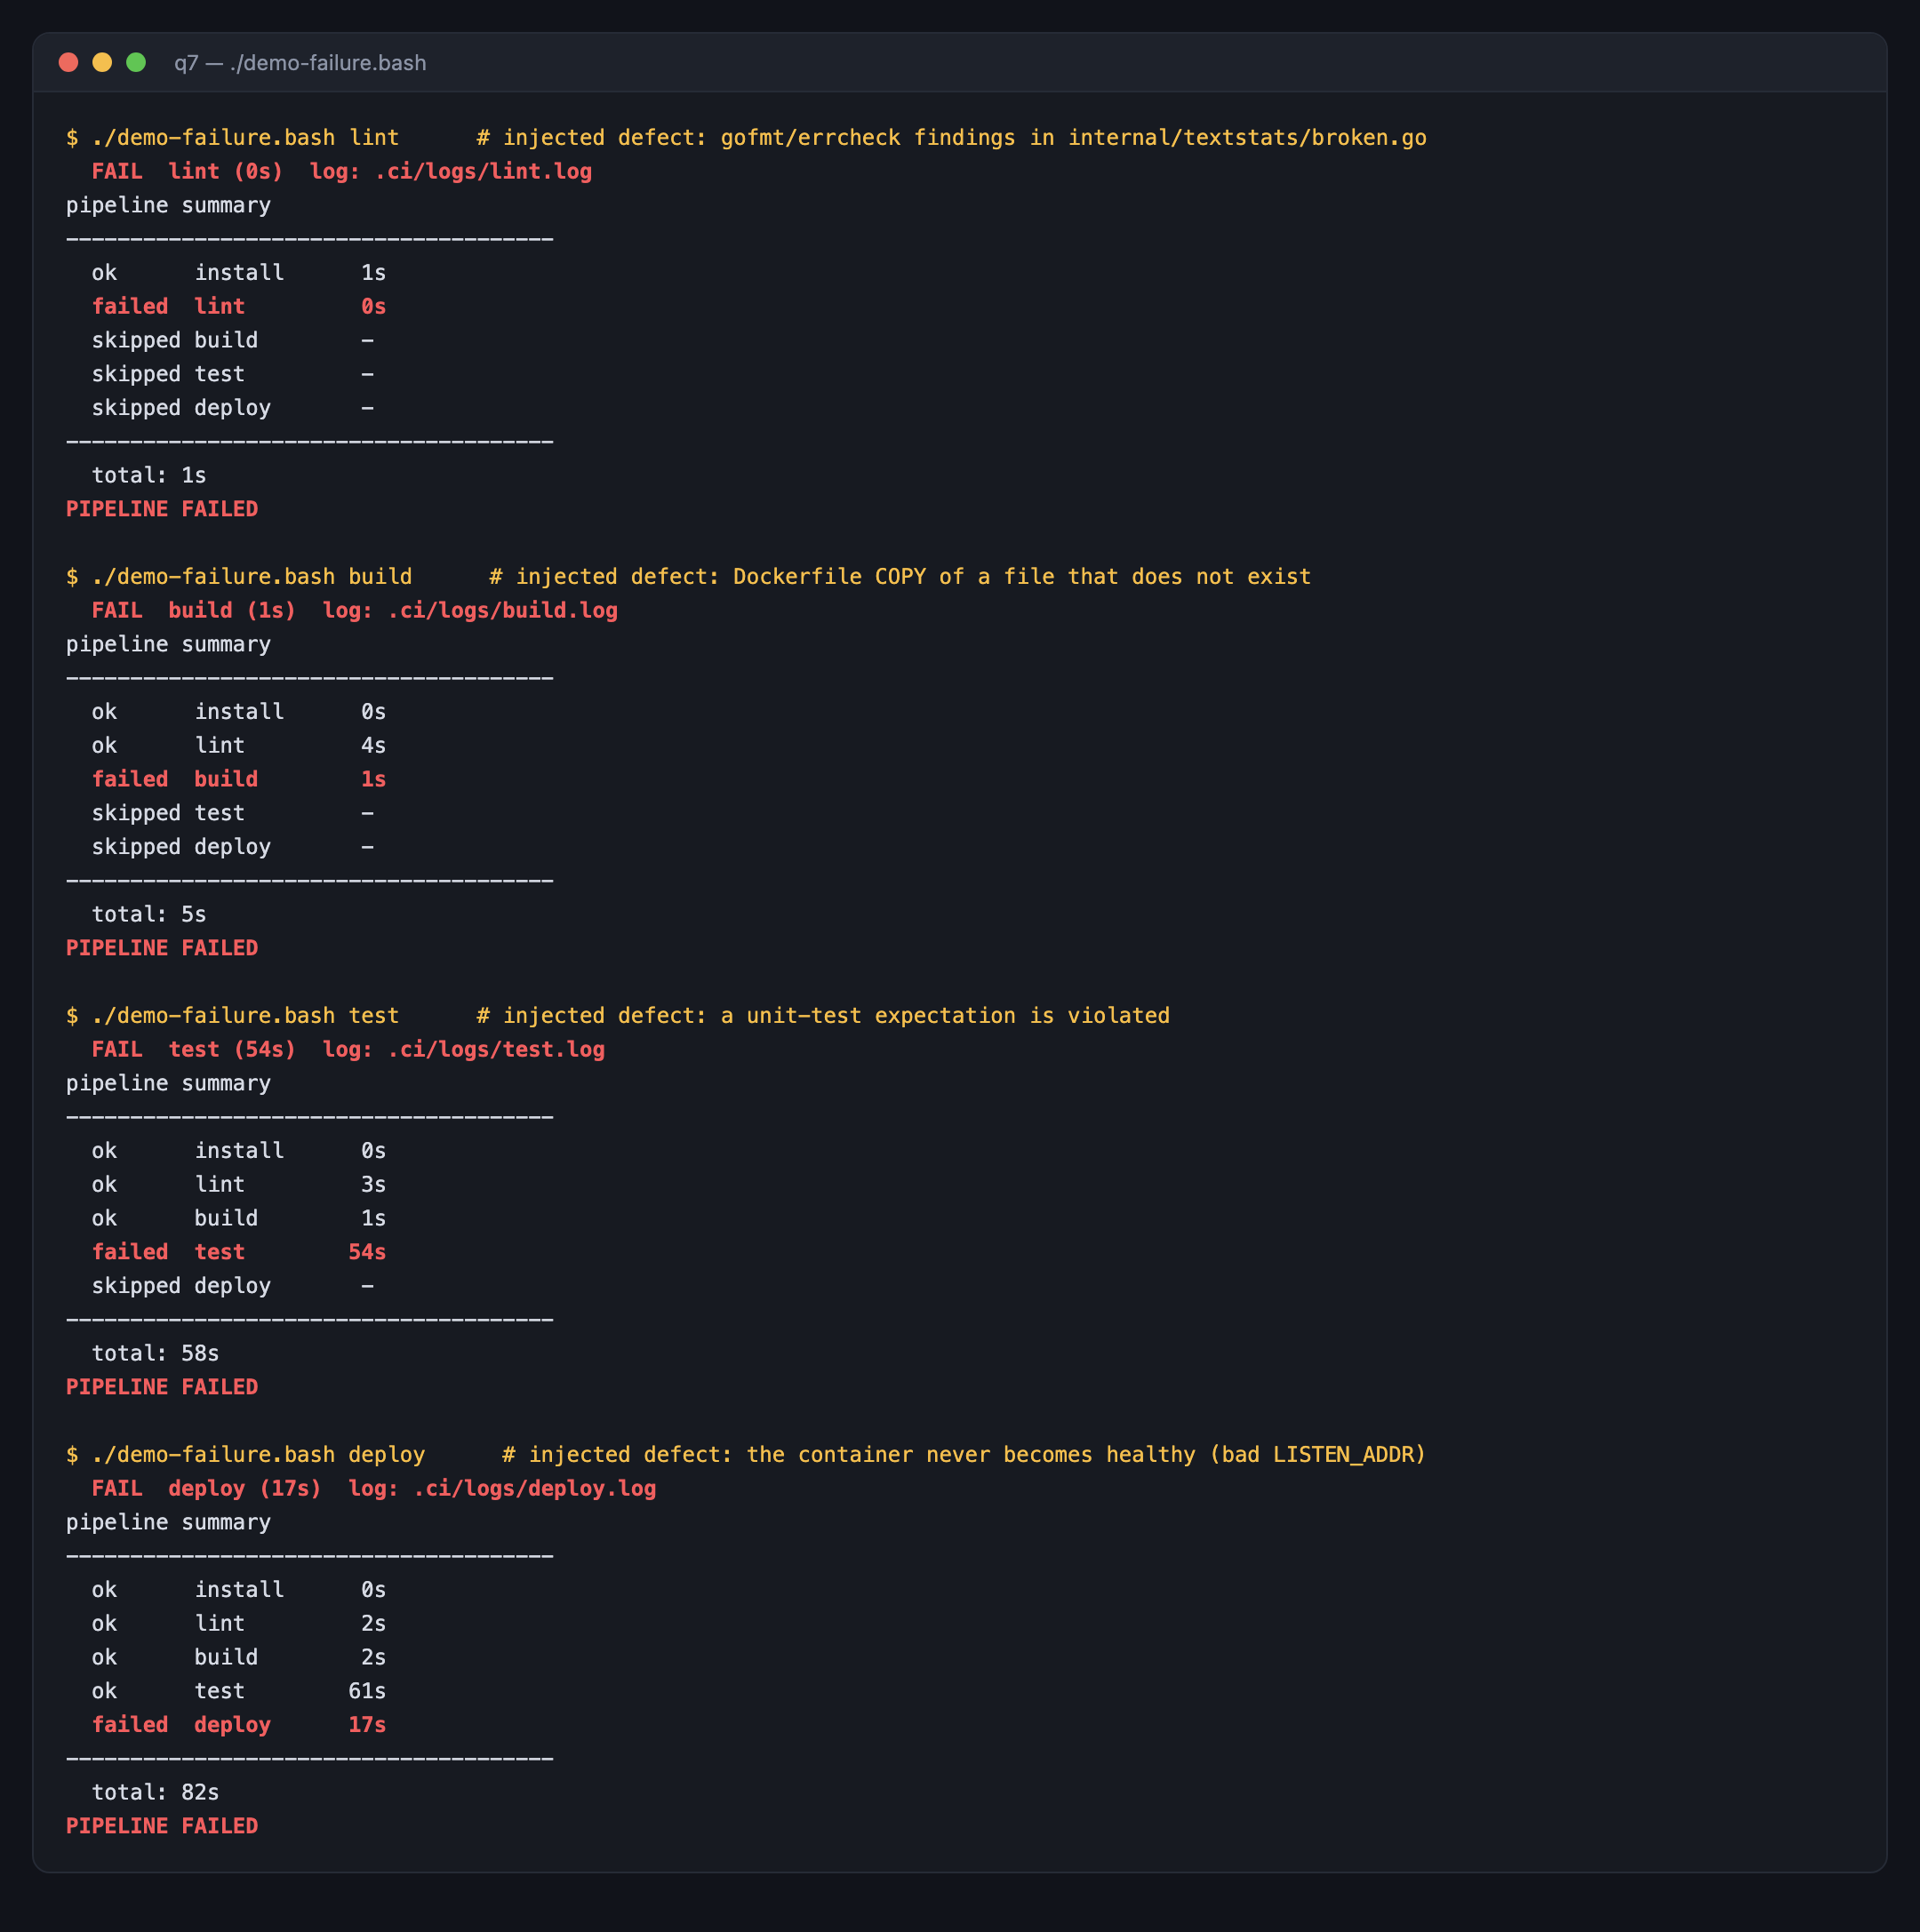
\includegraphics[width=0.95\textwidth]{figs/q7-fail.png}
\caption{در هر چهار حالت، جاب معیوب \lr{failed} می‌شود، جاب‌های بعدی \lr{skipped} می‌مانند و پایپلاین با کد غیرصفر خاتمه می‌یابد.}
\end{figure}
